%!TEX root = ./../main.tex
\section{Streaming Data}

Das Ziel unserer Aufgabenstellung ist die Verarbeitung von Streaming-Daten in Echtzeit. Die Streaming Data-Architektur
von Psaltis \cite{psaltis2017streaming} ist für diese Art von Problem konzipiert und bildet die Grundlage für
unsere Architektur. Nach der kurzen Vorstellung der Streaming Data-Architektur von Psaltis, zeigen wir unsere eigene konkrete
Umsetzung und vergleichen eingesetzten Technologien mit Alternativen.

\subsection{Streaming Data-Architektur nach Psaltis}

In \ref{fig:streaming_data_architecture-psaltis} sind die Komponenten der Streaming Data-Architektur, wie Psaltis \cite{psaltis2017streaming}
sie entwickelt hat. Der Collection Tier ist der Einstiegspunkt, der Daten in das System bringt. Unabhängig von dem verwendeten
Protokoll, werden die Daten mithilfe eines dieser Patterns übertragen \cite{psaltis2017streaming}:
\begin{itemize}
    \item Request/response pattern
    \item Publish/subscribe pattern
    \item One-way pattern
    \item Request/acknowledge pattern
    \item Stream pattern
\end{itemize}

Bei der Datenquelle kann es sich sowohl um von Hardware und auch von Software generierte Events handeln. Beispiele hierfür sind
Temperatur, Lautstärke oder auch Browser-Clicks.

\begin{figure}[h]
    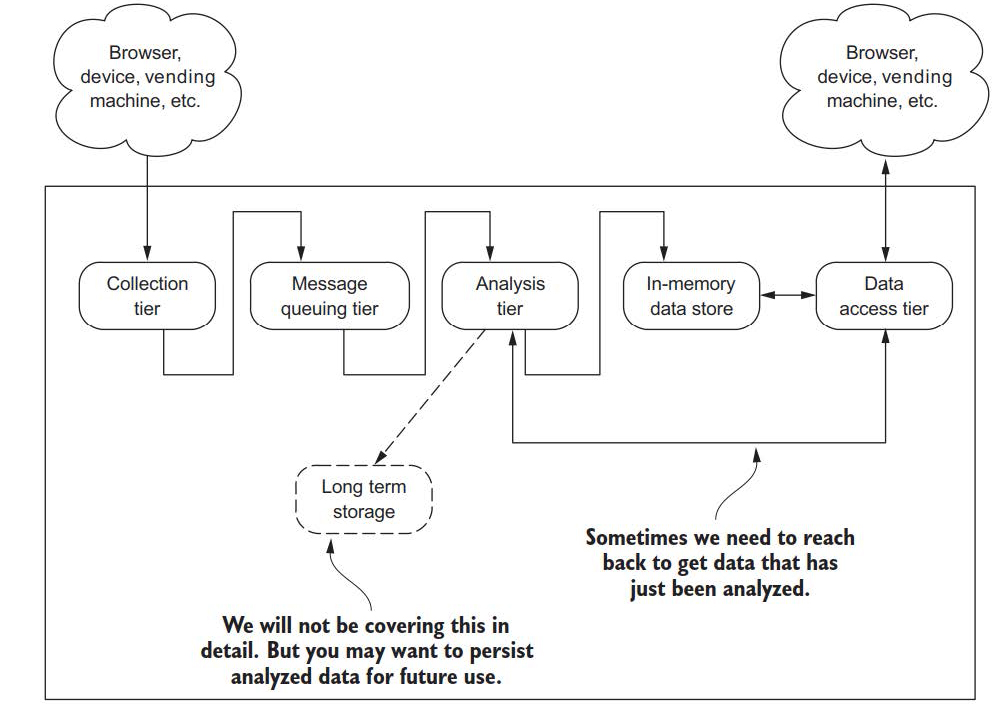
\includegraphics[width=.5\textwidth]{images/streaming_data_architecture-psaltis.jpg}
    \caption{Streaming Data-Architektur \cite{psaltis2017streaming}}
    \label{fig:streaming_data_architecture-psaltis}
\end{figure}

Um die Daten vom Collection Tier auf den Rest der Pipeline zu verteilen wird ein Messaging Queueing Tier implementiert.
Das Message Queueing Model ist ein Modell zur Interprozesskommunikation. Anwendungen schicken
Nachrichten an eine Nachrichtenschlange, von der andere Anwendnungen diese abholen können\cite{gray2003interprocess}.
Dadurch werden die eingesetzten Systeme voneinander entkoppelt und die Kommunikation findet nicht durch direkte Aufrufe,
sondern über die Queue statt \cite{psaltis2017streaming}. Im vorliegenden Fall wird der Collection Tier vom Rest der Pipeline entkoppelt.


\subsection{Konkrete Implementierung unserer Streaming Data-Architektur}
Die obigen vier Stufen der Streaming Data-Architektur von Psaltis \cite{psaltis2017streaming}
haben wir mit den folgenden konkreten Technologien besetzt, um die Aufgabenstellung aus dem vorhergehenden Kapitel zu erfüllen.
In diesem Kapitel geht es um die Frage, wieso wir uns für konkrete Technologien entschieden haben und im nachfolgenden Kapitel
stellen wir die Implementierungsdetails vor.
\begin{itemize}
    \item \textit{Collection tier.} Wikipedia ist unsere Datenquelle.
    Welches Pattern verwenden wir und wieso? Wie funktioniert das Pattern genau: siehe Psaltis https://goo.gl/qkgB8z
    \item \textit{Messaging queuing tier.} Wir nutzen ein Kafka-System: Weshalb Kafka? Welche Features
    (Durable messaging, Different Messaging Systems, Scalability, Performance, Transaction Support, Security, ...) sind für uns von großer Relevanz?
    Oder soll Kafka ein eigenes Kapitel bekommen?
    \item \textit{Analysis tier.} Esper: warum / welche Features sind für uns von Relevanz? Wie sieht die Ausgabe nach der Analyse aus?
    \item \textit{Data access tier.} ???
\end{itemize}